\documentclass[11pt]{ltjsarticle}
\usepackage{luatexja-fontspec}
\usepackage{amsmath,amssymb}
\usepackage[margin=22mm]{geometry}
\usepackage{graphicx}
\usepackage{longtable,booktabs,array}
\usepackage{calc}
\usepackage{xcolor}
\usepackage{hyperref}
\hypersetup{colorlinks=true,linkcolor=blue,urlcolor=blue,citecolor=blue}
\makeatletter
\def\maxwidth{\ifdim\Gin@nat@width>\linewidth\linewidth\else\Gin@nat@width\fi}
\makeatother
\setkeys{Gin}{width=\maxwidth,keepaspectratio}
\setcounter{secnumdepth}{0}
\setlength{\parindent}{0pt}
\setlength{\parskip}{0.5em}
\providecommand{\tightlist}{\setlength{\itemsep}{0pt}\setlength{\parskip}{0pt}}
\providecommand{\pandocbounded}[1]{#1}
\providecommand{\real}[1]{#1}
\newcounter{none}
\begin{document}
\section{マジックコインのトイモデル ──
無名性の限界（0・1・2）と隠れた変数の否定を視覚化する}\label{ux30deux30b8ux30c3ux30afux30b3ux30a4ux30f3ux306eux30c8ux30a4ux30e2ux30c7ux30eb-ux7121ux540dux6027ux306eux9650ux754c012ux3068ux96a0ux308cux305fux5909ux6570ux306eux5426ux5b9aux3092ux8996ux899aux5316ux3059ux308b}

\textbf{著者：} 木原 範昭（ORCID: 0009-0004-6753-4020） \textbf{日付：}
2026年6月18日 \textbf{DOI（本版）：} 10.5281/zenodo.20741265 ／
\textbf{Concept DOI（全版）：} 10.5281/zenodo.20741264 ／
\textbf{Zenodo:} https://zenodo.org/records/20741265 \textbf{関連論文：}
「高い対称性の極限におけるスケールの対数写像とスケール・量子化の分離について」§0.5（Concept
DOI:
\href{https://doi.org/10.5281/zenodo.20740841}{10.5281/zenodo.20740841}）

\begin{center}\rule{0.5\linewidth}{0.5pt}\end{center}

\subsection{はじめに}\label{ux306fux3058ux3081ux306b}

本稿は、関連論文
§0.5「系の中と外（不可知と不変量）」で述べた二つの主張------

\begin{enumerate}
\def\labelenumi{\arabic{enumi}.}
\tightlist
\item
  \textbf{無名性の限界＝2}：系の中では 0 と 1 が区別できず、2 と 2
  以上も区別できない。
\item
  \textbf{隠れた変数の否定}：内側を全部見せても枚数を分離する手がかりは無い。
\end{enumerate}

------を、数式の前に体感できるよう、卓上マジックのトイモデルとして視覚化するものである。これは厳密な証明ではなく、\textbf{直感的な入口（イラストレーション）}である。

\begin{center}\rule{0.5\linewidth}{0.5pt}\end{center}

\subsection{装置の設定}\label{ux88c5ux7f6eux306eux8a2dux5b9a}

すべてのシーンで共通の卓上装置を用いる。

{\def\LTcaptype{none} % do not increment counter
\begin{longtable}[]{@{}
  >{\raggedright\arraybackslash}p{(\linewidth - 4\tabcolsep) * \real{0.3333}}
  >{\raggedright\arraybackslash}p{(\linewidth - 4\tabcolsep) * \real{0.3333}}
  >{\raggedright\arraybackslash}p{(\linewidth - 4\tabcolsep) * \real{0.3333}}@{}}
\toprule\noalign{}
\begin{minipage}[b]{\linewidth}\raggedright
装置
\end{minipage} & \begin{minipage}[b]{\linewidth}\raggedright
役割
\end{minipage} & \begin{minipage}[b]{\linewidth}\raggedright
対応する概念
\end{minipage} \\
\midrule\noalign{}
\endhead
\bottomrule\noalign{}
\endlastfoot
半透明のすりガラス調コップ & コインを入れる容器（中はうっすら見える） &
系そのもの \\
デジタル秤（重量計） & 外から測る客観的な観測量。1 枚 = 10g
で加法的に増える & \textbf{系の外（観測者）／保存量}（加法的な総量） \\
CRT モニター &
各コインに付いたカメラが映す像。\textbf{カメラは自分自身を映せず、他のコインだけを映す}
& \textbf{系の中（無名の内部視点）} \\
マジシャンの手 & コインを操作する（ゼロ調整・追加・ズル） & 操作者 \\
\end{longtable}
}

要点は、\textbf{モニター（系の中）と秤（系の外）を分けて見ること}である。モニターは無名の内部から「自分以外があるか」を映し、秤は外から加法的な総量を測る。本系は双対的で「どちらが実在か」は問わない。客観的な錨は実在ではなく、加法的に保存される総量（秤の値）と不動点に置く。

\begin{center}\rule{0.5\linewidth}{0.5pt}\end{center}

\subsection{Figure 1：ゼロ点調整 ── 0 と null
の区別不能}\label{figure-1ux30bcux30edux70b9ux8abfux6574-0-ux3068-null-ux306eux533aux5225ux4e0dux80fd}

\begin{figure}
\centering
\pandocbounded{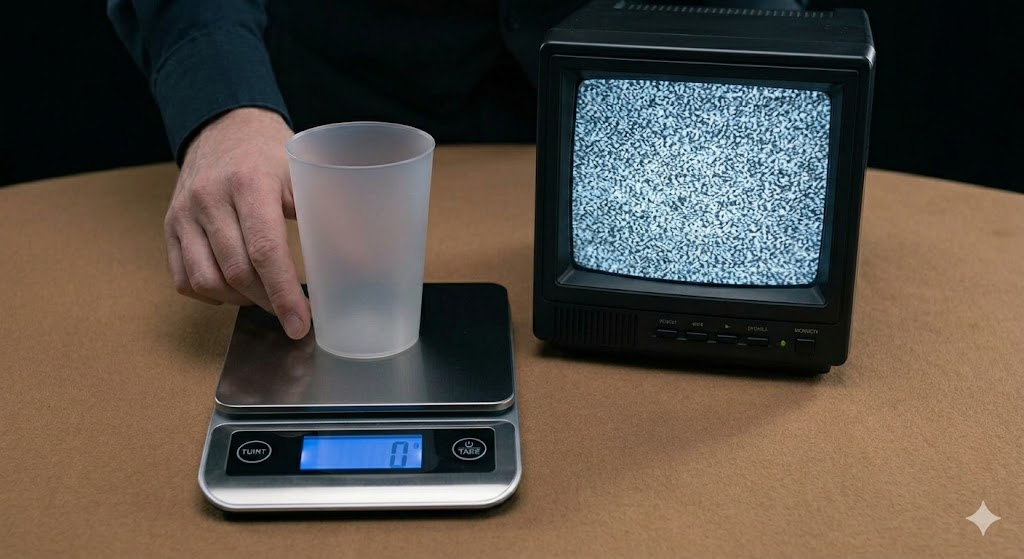
\includegraphics[keepaspectratio,alt={Figure 1}]{FIg1.jpeg}}
\caption{Figure 1}
\end{figure}

\begin{itemize}
\tightlist
\item
  \textbf{系（モニター）：} 砂嵐。何も無い（null）。コップの内壁だけ。
\item
  \textbf{観測（秤）：} 0g（マジシャンがゼロ調整＝tare した状態）。
\end{itemize}

\textbf{対応：} 状態を判断する主体がそもそも無い。ゆえに \textbf{0 は
null
と区別できない}。秤のゼロという具体物が、「無」と「ゼロ」が同じに見えることを示す。これは
0 が実在しないという意味ではなく、内部から区別できないという意味である。

\begin{center}\rule{0.5\linewidth}{0.5pt}\end{center}

\subsection{Figure 2：1 枚目のコイン ── 1 は 0
と区別できない}\label{figure-21-ux679aux76eeux306eux30b3ux30a4ux30f3-1-ux306f-0-ux3068ux533aux5225ux3067ux304dux306aux3044}

\begin{figure}
\centering
\pandocbounded{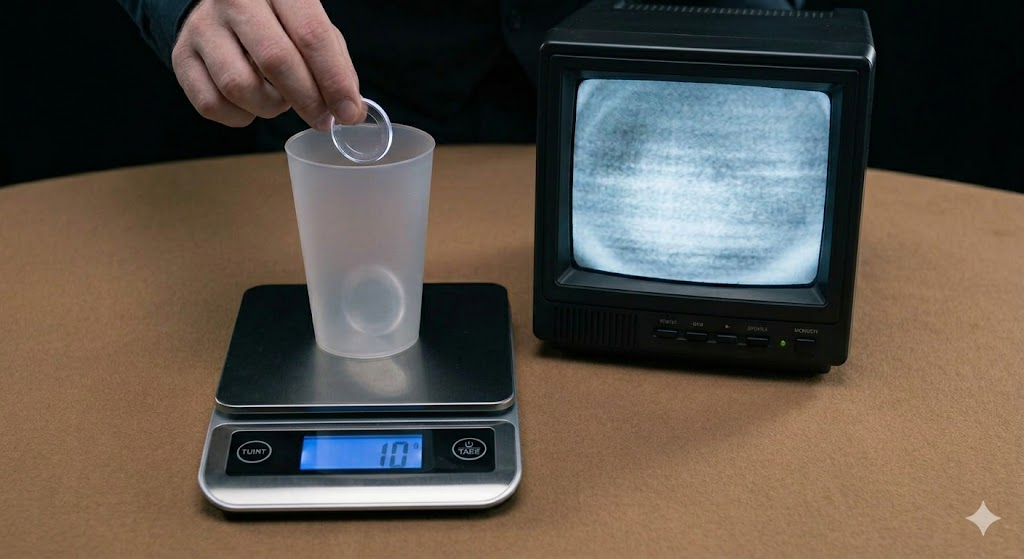
\includegraphics[keepaspectratio,alt={Figure 2}]{Fig2.jpeg}}
\caption{Figure 2}
\end{figure}

\begin{itemize}
\tightlist
\item
  \textbf{系（モニター）：}
  ほとんど信号が立たない（薄くにじむのみ）。唯一のコインのカメラには\textbf{映すべき「自分以外」が無い}ため、自分自身を捉えられない。
\item
  \textbf{観測（秤）：} 10g。コップにはうっすらコインが 1 枚見える。
\end{itemize}

\textbf{対応：}
比較する相手がいないため、内部では「自分がいる」ことが確定できない。ゆえに
\textbf{系の中では 1 は 0 と区別できない}。一方、秤（系の外）は 10g
を示す------\textbf{外の保存量は増えているのに、内部の像は立たない}。この食い違いが、系の中と外の分離そのものである。

\begin{center}\rule{0.5\linewidth}{0.5pt}\end{center}

\subsection{Figure 3：2 枚目のコイン ── 2
で差異が立つ}\label{figure-32-ux679aux76eeux306eux30b3ux30a4ux30f3-2-ux3067ux5deeux7570ux304cux7acbux3064}

\begin{figure}
\centering
\pandocbounded{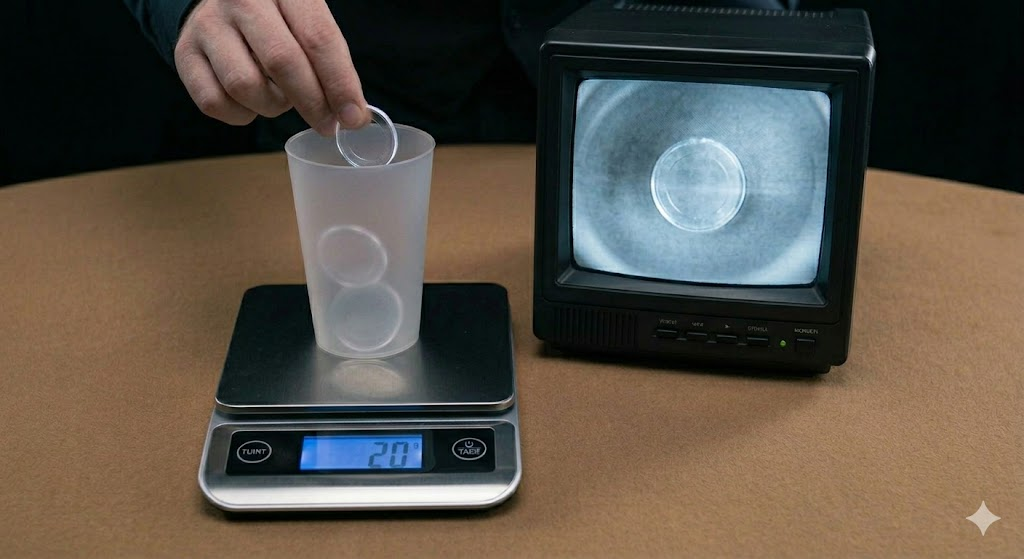
\includegraphics[keepaspectratio,alt={Figure 3}]{Fig3.jpeg}}
\caption{Figure 3}
\end{figure}

\begin{itemize}
\tightlist
\item
  \textbf{系（モニター）：} \textbf{ONE（1
  枚）}の透明なコインが、初めて明瞭に映る。一方のコインのカメラが、もう一方を捉えたためである。
\item
  \textbf{観測（秤）：} 20g。コップにはコインが 2 枚。
\end{itemize}

\textbf{対応：}
初めて「自分以外」が現れ、それを通じて「自分がいる」が立つ。\textbf{2
が、系の中から何かが知れる最小}である。モニターに「1
枚」が映ること------すなわち系の中で初めて「1（＝一つの他者）」が発生すること------が、差異の成立の正体である。外（秤）は
20g、内（モニター）は「他者 1」。

\begin{center}\rule{0.5\linewidth}{0.5pt}\end{center}

\subsection{Figure 4：3 枚目のコイン ── 2 と 2
以上は区別できない（隠れた変数の否定）}\label{figure-43-ux679aux76eeux306eux30b3ux30a4ux30f3-2-ux3068-2-ux4ee5ux4e0aux306fux533aux5225ux3067ux304dux306aux3044ux96a0ux308cux305fux5909ux6570ux306eux5426ux5b9a}

\begin{figure}
\centering
\pandocbounded{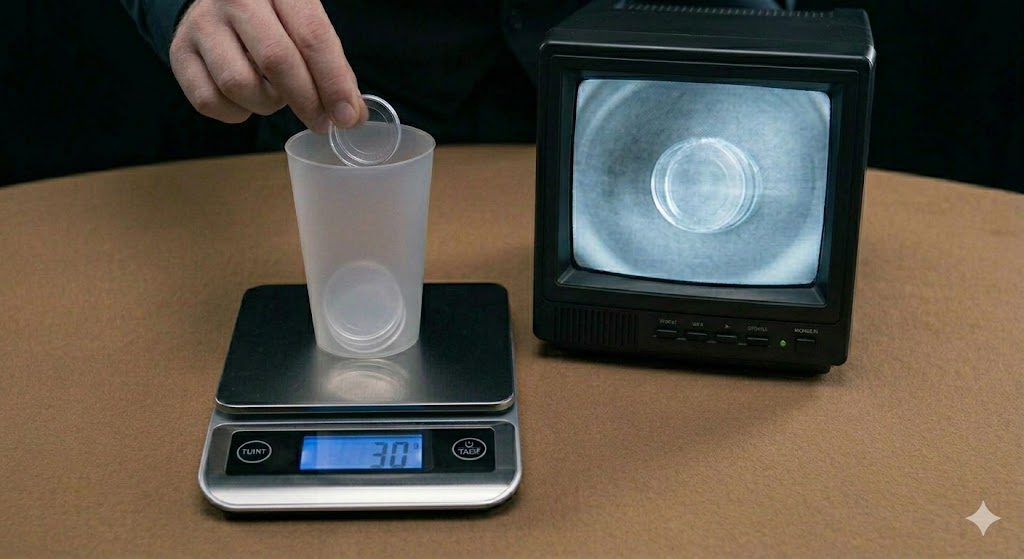
\includegraphics[keepaspectratio,alt={Figure 4}]{Fig4.jpeg}}
\caption{Figure 4}
\end{figure}

\begin{itemize}
\tightlist
\item
  \textbf{系（モニター）：} 依然として \textbf{ONE（1
  枚）}のまま。しかしよく見ると\textbf{二重の輪郭（ダブルエッジ）}が現れ、像がわずかにブレている。マジシャンが少しズラして重ねた「ズル」の痕跡である。
\item
  \textbf{観測（秤）：}
  30g。コップには、ズレて重ねられたコイン形状（厚いスタック）。
\end{itemize}

\textbf{対応：} 内部のカメラは「他者がある」までしか映せず、それが 2
枚なのか 3 枚なのかを分離できない。ゆえに \textbf{系の中では 2 と 2
以上は区別できない}。ダブルエッジは唯一の手がかりだが、枚数を確定する情報にはならない------\textbf{内側から全部見せても分からない}。これが\textbf{隠れた変数の否定}である：内部に「本当の枚数」という隠れた変数があって観測精度で見えないのではなく、内部の視点には枚数を分離する構造がそもそも無い。

（秤は 30g を示し、加法的な保存量としては 3
単位ぶんが立つ。これは系の外の客観的な錨であり、系の中の不可知を否定しない。\textbf{外の保存量は数えられるが、内の像は数えられない}------この非対称こそが本トイモデルの核である。）

\begin{center}\rule{0.5\linewidth}{0.5pt}\end{center}

\subsection{まとめ ──
一枚の表}\label{ux307eux3068ux3081-ux4e00ux679aux306eux8868}

{\def\LTcaptype{none} % do not increment counter
\begin{longtable}[]{@{}
  >{\raggedright\arraybackslash}p{(\linewidth - 6\tabcolsep) * \real{0.2500}}
  >{\raggedright\arraybackslash}p{(\linewidth - 6\tabcolsep) * \real{0.2500}}
  >{\raggedright\arraybackslash}p{(\linewidth - 6\tabcolsep) * \real{0.2500}}
  >{\raggedright\arraybackslash}p{(\linewidth - 6\tabcolsep) * \real{0.2500}}@{}}
\toprule\noalign{}
\begin{minipage}[b]{\linewidth}\raggedright
Fig
\end{minipage} & \begin{minipage}[b]{\linewidth}\raggedright
秤（系の外・保存量）
\end{minipage} & \begin{minipage}[b]{\linewidth}\raggedright
モニター（系の中・不可知）
\end{minipage} & \begin{minipage}[b]{\linewidth}\raggedright
示すこと
\end{minipage} \\
\midrule\noalign{}
\endhead
\bottomrule\noalign{}
\endlastfoot
1 & 0g & null（砂嵐） & 0 と null は区別できない \\
2 & 10g & 立たない & 1 は 0 と区別できない \\
3 & 20g & 他者 1 が明瞭 & 2 で差異が立つ（系の中の「1」の発生） \\
4 & 30g & 他者 1（二重輪郭） & 2 と 2
以上は区別できない（隠れた変数の否定） \\
\end{longtable}
}

系の外（秤）では量が 0,10,20,30
と加法的に保存・増加する一方、系の中（モニター）の像は \textbf{null →
立たない → 他者1 → 他者1（分離不能）} と、2
を天井に飽和する。\textbf{保存量（外）は数えられ、無名の内部像は数えられない}------関連論文
§0.5
の「無名性の限界＝2」と「内部の不可知は外の整数構造を否定しない」が、そのまま卓上で再現される。

\begin{center}\rule{0.5\linewidth}{0.5pt}\end{center}

\subsection{このモデルの限界（読み解きの注意）}\label{ux3053ux306eux30e2ux30c7ux30ebux306eux9650ux754cux8aadux307fux89e3ux304dux306eux6ce8ux610f}

本稿は厳密な証明ではなく、§0.5
の存在論を体感するための\textbf{イラストレーション}である。トイモデルゆえの単純化があり、厳密に詰めるほど難解になる。以下は、誤読を避けるための注意であって、モデルを精密化するものではない。

\begin{enumerate}
\def\labelenumi{\arabic{enumi}.}
\item
  \textbf{モニターは「一つの無名要素の一人称視点」である。}
  神の視点の総数ではない。だから 2 枚でも画面は「他者が
  1」しか映らない（各コインから見えるのは自分以外の 1
  枚だから）。Fig3・Fig4 の「ONE」は「他者が present
  になった」ことの像であって、内部が枚数を数え始めたわけではない。
\item
  \textbf{秤は「枚数」ではなく加法的な総量（スカラー）を読むだけである。}
  30g から「3 枚」を出すには「1 枚 = 10g
  で全部同一」という\textbf{外からの仮定}が要る。その同一性こそ無名性が内部に許さないものなので、秤も枚数を直接「見て」はいない。秤が客観的に立つのは加法的な総量であって、内部の不可知と矛盾しない。本トイモデルの主眼は、\textbf{内の不可知と外の総量の非対称}を見せることにある。
\item
  \textbf{ここでの「隠れた変数の否定」は Bell の定理の意味ではない。}
  EPR/Bell の no-hidden-variables
  とは別物で、「内部の視点に枚数を分離する構造がそもそも無い」という弱い意味に限る。
\item
  \textbf{本トイモデルが扱うのは §0.5 の一部である。} 「0・1・2
  の区別不能」と「枚数分離の不在」を可視化するもので、双対・共役（「ν と
  λ のどちらが実在か」は問えない）は図には含まれない。
\item
  \textbf{物理的同定は行わない。} コインが何を表すかは扱わない。
\end{enumerate}

\begin{center}\rule{0.5\linewidth}{0.5pt}\end{center}

\subsection{参照}\label{ux53c2ux7167}

\begin{itemize}
\tightlist
\item
  Kihara, N.
  「高い対称性の極限におけるスケールの対数写像とスケール・量子化の分離について
  ── 最小公理系からの限定的検証報告（改訂版）」§0.5。Concept DOI:
  \href{https://doi.org/10.5281/zenodo.20740841}{10.5281/zenodo.20740841}，v1
  DOI:
  \href{https://doi.org/10.5281/zenodo.20740842}{10.5281/zenodo.20740842}。
\end{itemize}
\end{document}
